\documentclass[aspectratio=43]{beamer}
\usetheme{Madrid}
\usepackage[english]{babel}
\usepackage[font=small,labelfont=bf]{caption}
\title{ETG Turbulence Isotropization}
\author[S. Tirkas]{Stefan Tirkas\inst{1}\texorpdfstring{\\}\and Hoatian Chen\inst{1}\and Gabriele Merlo\inst{2}\and Scott Parker\inst{1}}
\institute[CIPS]{
    \inst{1}CIPS, University of Colorado, Boulder\and
    \inst{2}University of Texas, Austin
} 
\date{\today}
\logo{
\includegraphics[width=.2\linewidth]{Images/BoulderLogo.png}}

\begin{document}
    
   \frame{\titlepage}
   
   \begin{frame}{Outline}
       \tableofcontents
   \end{frame}
   
   \section{Drift Wave Instabilities}
   
   \begin{frame}{Drift Wave Instabilities}
      \begin{itemize}
         \item Drift waves are characterized as density, temperature or pressure fluctuations in plasmas. Mostly simply they are involved electrostatically
         in low-$\beta$ plasmas.
         \vspace{5mm}
         \item Modes relevant to tokamak physics include ion-temperature-gradient modes (ITG), electron-temperature-gradient 
         modes (ETG), and trapped electron modes (TEM).
         \vspace{5mm}
         \item Low-frequency drift wave turbulence is largely responsible for the anomalous transport of plasma particles
         across magnetic field lines.
      \end{itemize}
   \end{frame}

   \begin{frame}{Ion-Temperature-Gradient Mode Growth}
      \begin{figure}
         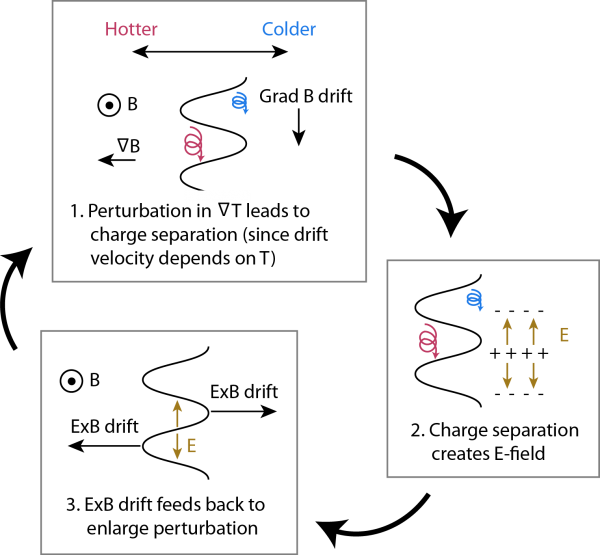
\includegraphics[scale=0.3]{Images/ITG_Instability.png}
         \caption{Simple picture of ITG instability.}
      \end{figure}
   \end{frame}

   \begin{frame}{ETG Simulation in GENE}
      \begin{columns}
      \column{0.6\textwidth}
         \begin{figure}
            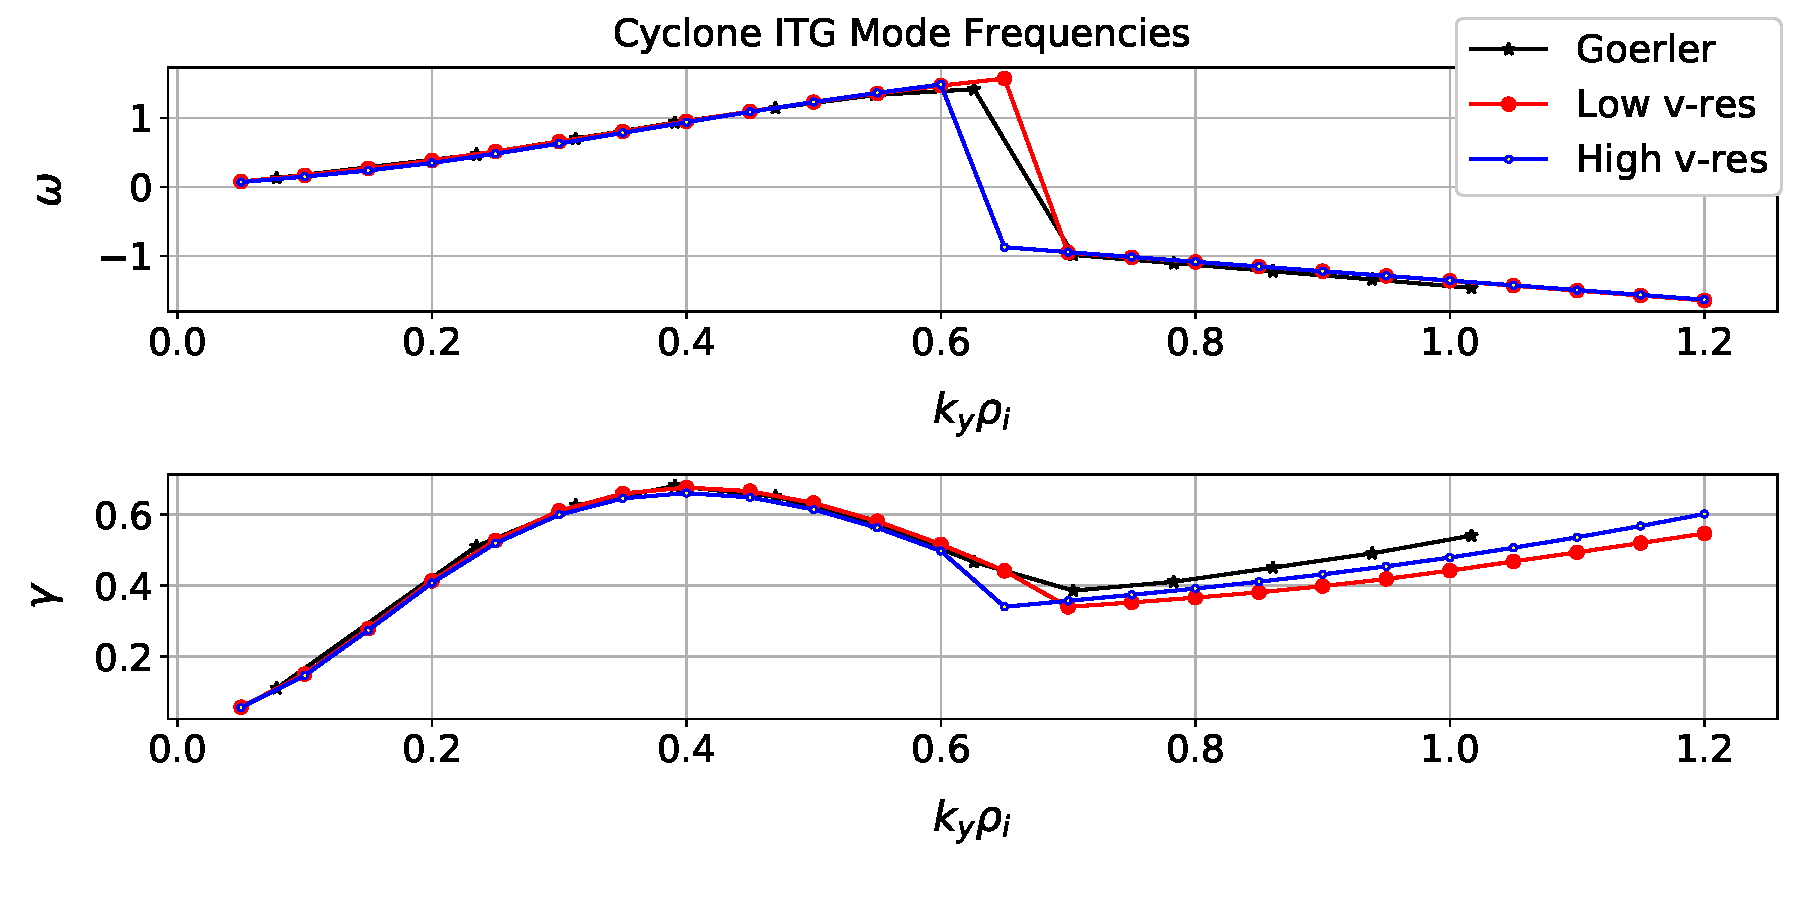
\includegraphics[width=.8\textwidth,height=.3\textheight]{Images/LinearITG_KinEl_GrowthRates.pdf}
            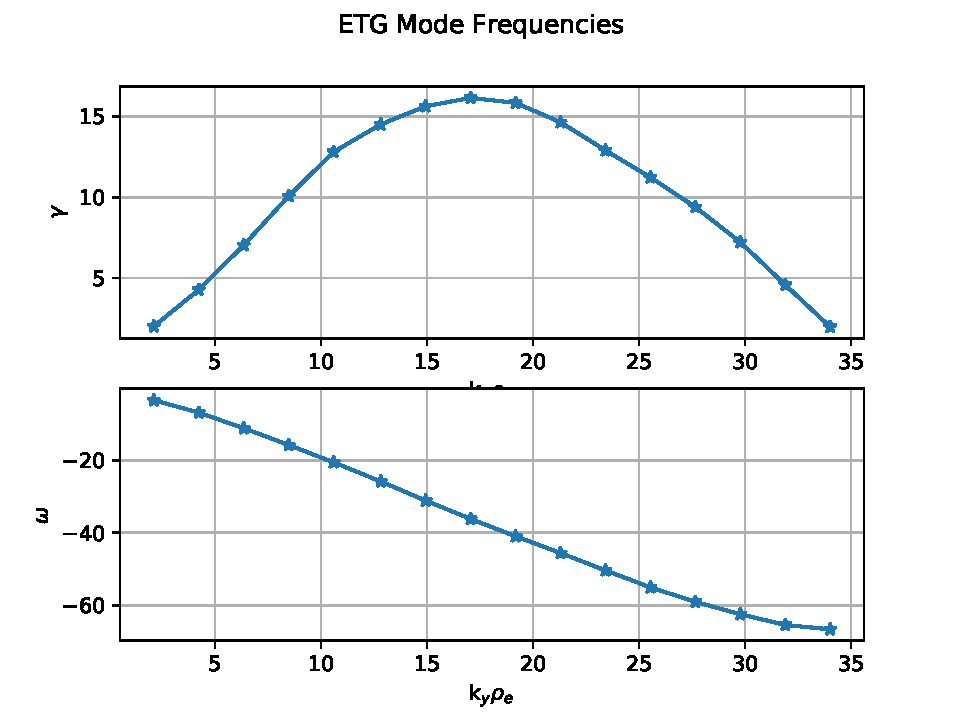
\includegraphics[width=.8\textwidth]{Images/GrowthRates_ETG.pdf}
         \end{figure}
      \column{0.4\textwidth}
         \begin{itemize}
            \item Successful reproduction of Goerler benchmark with kinetic ions and electrons, showing ITG mode and trapped electron mode growth.
            \item Conversion of ITG to ETG flux-tube case prior to running non-linear simulations.
         \end{itemize}
      \end{columns}
   \end{frame}

   \begin{frame}{ETG "Streamers" in GENE}
      \begin{columns}
      \column{0.5\textwidth}
         \begin{figure}
            \hspace*{-.3cm}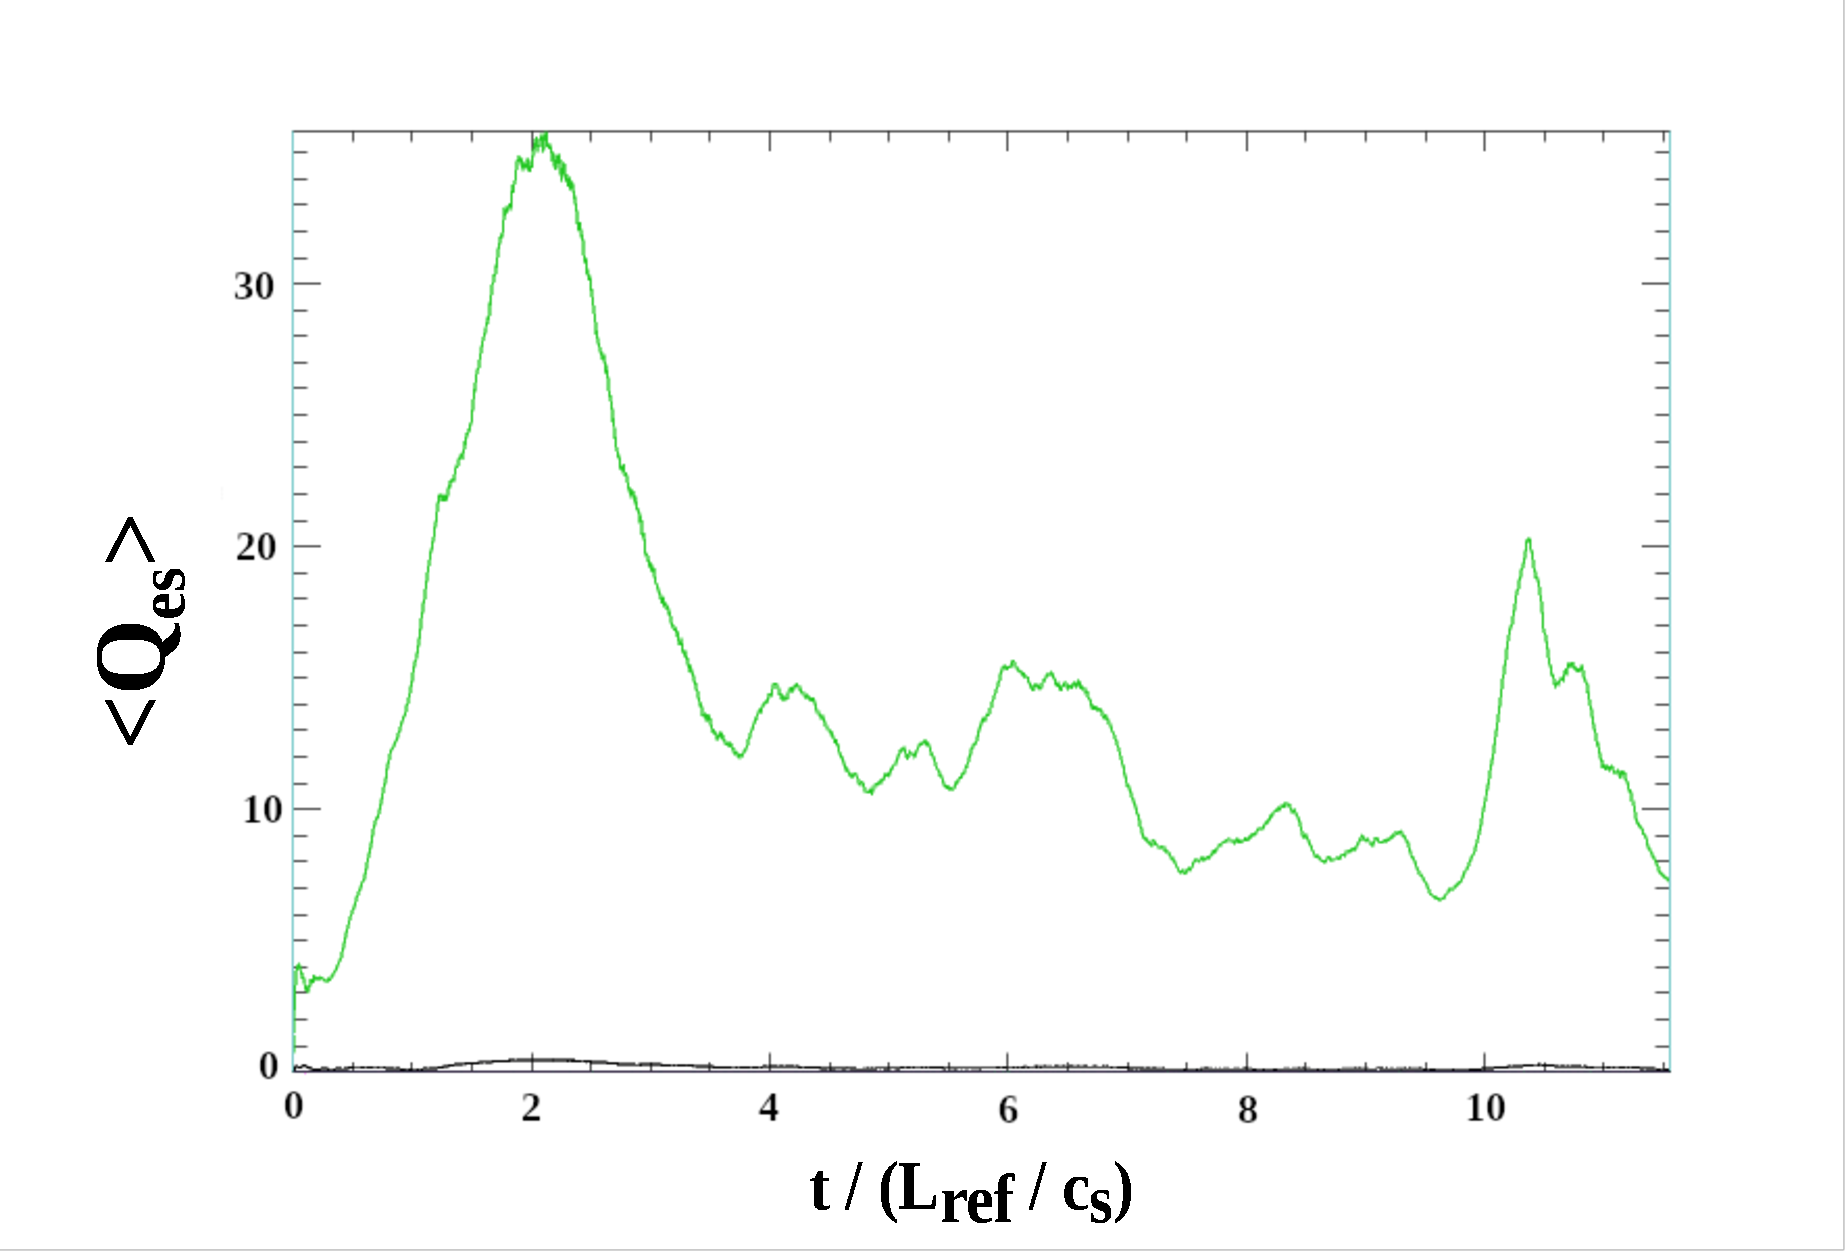
\includegraphics[scale=.2]{Images/etgHeatFlux.pdf}
            \hspace*{-.3cm}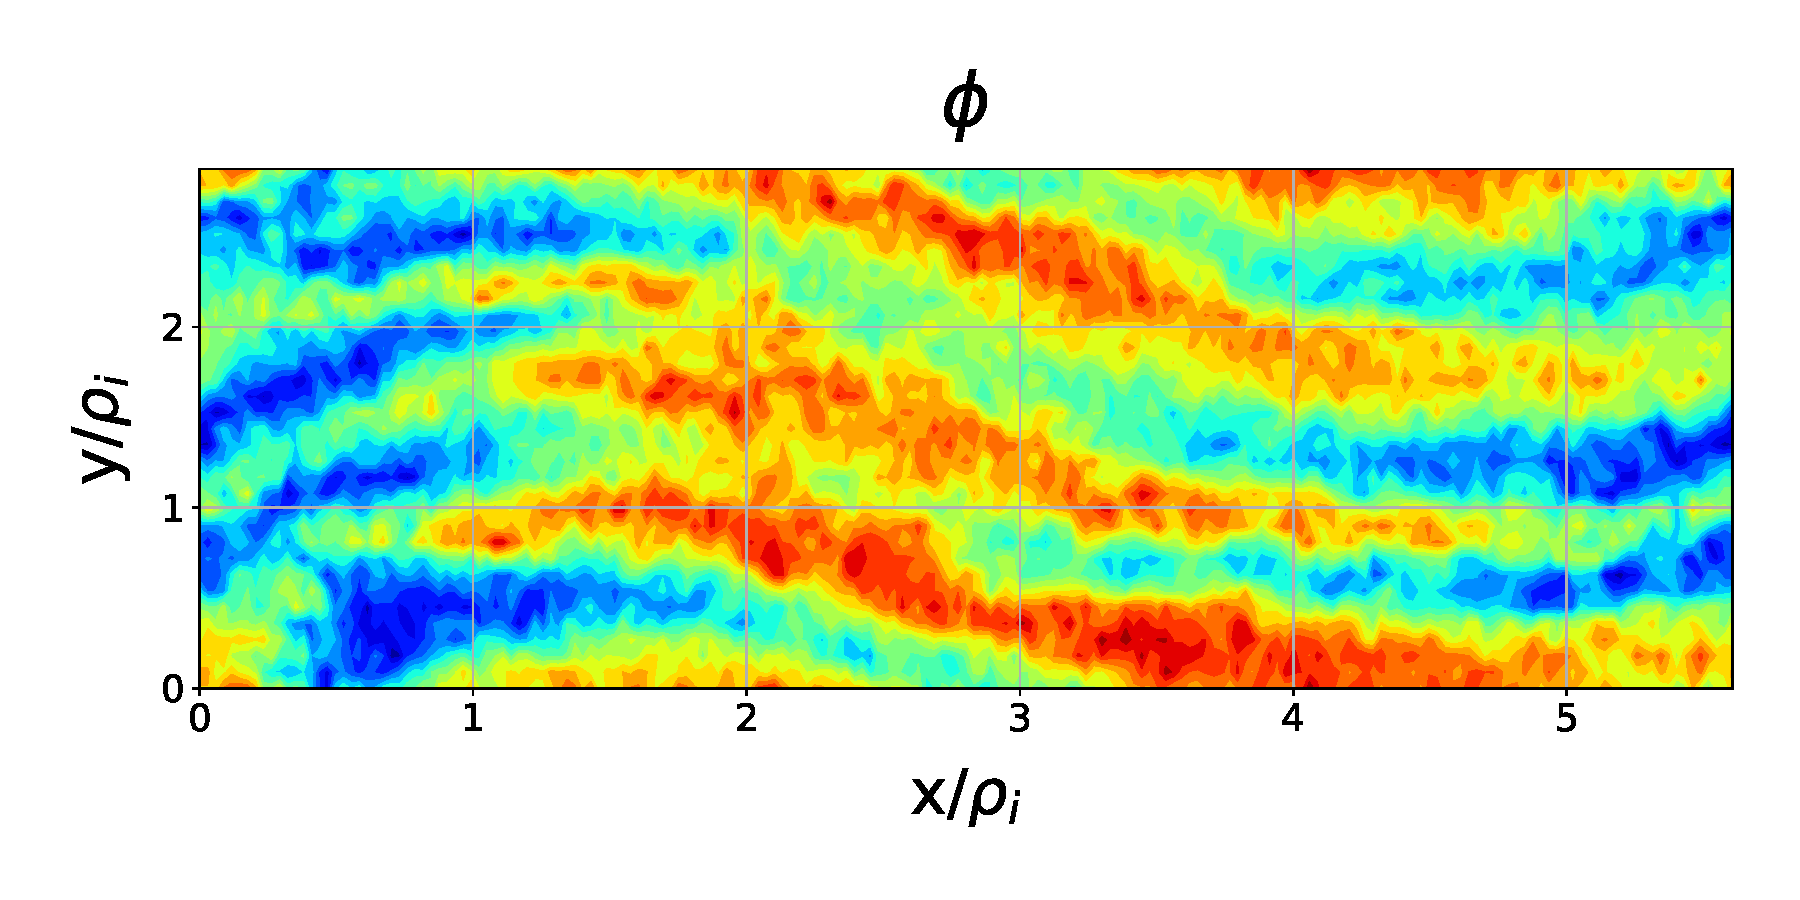
\includegraphics[scale=.2]{Images/genePhiETG_sat2.pdf}
         \end{figure}
      \column{0.5\textwidth}
         \begin{itemize}
            \item ETG turbulence in toroidal gyrokinetic simulations is associated with elongated "streamers".
            \item Multiscale turbulence simulations have shown that streamers dominate electron heat flux and lead
            best reproduced experimental heat fluxes within experimental uncertainties.
         \end{itemize}
      \end{columns}
   \end{frame}

   \section{Hasegawa-Mima Fluid Model}

   \begin{frame}{Hasegawa-Mima Fluid ETG Model}
      \begin{itemize}
         \item Partial differential equation derived from fluid continuity and momentum equations.
         \item Approximations made that are useful to describing  turbulence in tokamak plasmas.
         \begin{itemize}
            \item Cyclotron motion periods much smaller than time scales that quantities of interest change on ($B$,$\Phi$,$n$).
            \item Long length scales along $\hat{b}$-direction - $k_{\parallel}/k_{\perp}\equiv\epsilon\ll1$.
            \item Quasi-neutrality of particle densities is enforced.
            \item Isothermal equation of state, with adiabatic ions that have negligible temperatures.
         \end{itemize}
         \item Shown to cause isotropic behavior for long wavelength modes as well as an inverse energy-cascade.
      \end{itemize}
   \end{frame}

   \begin{frame}{Hasegawa-Mima Equations}
      \quad We start with the fluid continuity and momentum equations and $\tau = T_e/T_i$, where we have already taken the ion approximations discussed
   on the previous slide:
      \begin{equation}
         \frac{\partial n_e}{\partial t} + \nabla\cdot\left(n_e\vec{v}_e\right) = 0,
      \end{equation}
      %
      \begin{equation}
            m_e\frac{d\vec{v}_e}{dt} = \left(1+\tau\right)e\nabla\delta\Phi - \frac{e}{c}\vec{v}_e\times\vec{B}-\frac{\nabla P_e}{n_e}\;.
      \end{equation}
      \quad We break equation (2) up into parallel and perpendicular components by taking a dot product with $\hat{b}$ to find,
      \begin{equation}
         \frac{d\vec{v}_{e,\parallel}}{dt} = (1+\tau)\frac{e}{m_e}\partial_t^{-1}\nabla_{\parallel}\delta\Phi \Rightarrow v_{\parallel}
            \simeq (1+\tau)\frac{k_{\parallel}e\delta\Phi}{m_e\omega},
      \end{equation}
   \end{frame}

   \begin{frame}{Hasegawa-Mima Equations}
      \begin{equation}
         \frac{d\vec{v}_{e,\perp}}{dt} = (1+\tau)\frac{e}{m_e}\nabla_{\perp}\delta\Phi - \omega_{c,e}\vec{v}_{e,\perp}-\frac{\hat{b}\times\nabla P_e}{m_en_e}\;.
      \end{equation}
      \quad Then we can split up $\vec{v}_e$ by ordering
      \begin{equation}
      \begin{aligned}
         \vec{v}_{e,0} &= \vec{v}_{\parallel} + \vec{v}_{\perp,0} = \vec{v}_{\parallel} + \left(1 + \tau\right)\vec{v}_E + \vec{v}_D,  \\
         \vec{v}_{e,1} &= \vec{v}_{\perp,1} = -\frac{1}{\omega_{c,e}}(\partial_t+\vec{v}_{e,0}\cdot\nabla)(\hat{b}\times\vec{v}_{e,0}) \\
                       &\simeq \frac{e(1+\tau)}{m_e\omega_{c,e}^2}\partial_t\nabla_{\perp}\delta\Phi - [\frac{\vec{b}\times\nabla P_e}{n_e}\cdot\nabla_{\perp}]
                               \frac{e(1+\tau)}{m_e^2\omega_{c,e}^3}\nabla_{\perp}\delta\Phi \\
                       &+      \frac{e^2(1+\tau)^2}{m_e^2\omega_{c,e}^3}[\hat{b}\times\nabla_{\perp}\Phi\cdot\nabla_{\perp}]\nabla_{\perp}\delta\Phi\;.
      \end{aligned}
      \end{equation}
   \end{frame}

   \begin{frame}{Hasegawa-Mima Equations}
      \quad Now, with incompressibility, $\nabla\cdot\vec{v}_{e,0,\perp}=0$, equation (1) becomes,
      \begin{equation}
         \partial_t\delta n_e+n_e\nabla\cdot(v_{\parallel} + \vec{v}_{e,1}) + \nabla\delta n_e\cdot\vec{v}_D+(1+\tau)\delta n_e\cdot\vec{v}_E = 0,
      \end{equation}
      and plugging in $\delta n_e=\delta n_i$, we find that to order $\epsilon$,
      \begin{equation}
      \begin{aligned}
         &-n_e\partial_t\frac{e\delta\Phi}{T_i} + n_e(1+\tau)\frac{e}{m_e}\partial_t^{-1}\nabla_{\parallel}^2\delta\Phi
         + \frac{en_e(1+\tau)}{m_e\omega_{c,e}^2}\partial_t\nabla_{\perp}^2\delta\Phi \\
         &- \frac{e(1+\tau)}{m_e^2\omega_{c,e}^3}[\hat{b}\times\nabla P_e\cdot\nabla_{\perp}]\nabla_{\perp}^2\delta\Phi
         + \frac{e^2n_e(1+\tau)^2}{m_e^2\omega_{c,e}^3}[\hat{b}\times\nabla_{\perp}\delta\Phi\cdot\nabla_{\perp}]\nabla_{\perp}^2\delta\Phi \\
         &+ \nabla_{\perp}\frac{e\delta\Phi}{T_i}\cdot\frac{\hat{b}\times\nabla P_e}{m_e\omega_{c,e}} + (1+\tau)\frac{e}{m_e\omega_{c,e}}\nabla n_e\cdot\hat{b}\times\nabla\Phi = 0\;.
      \end{aligned}
      \end{equation}
   \end{frame}

   \begin{frame}{Hasegawa-Mima Equations}
      \quad Taking the standard electron dyanamic normalization,
      \begin{equation}
      \begin{aligned}
         \Phi    = \frac{e\delta\Phi}{T_i},&\; -\frac{1}{r_n}=\frac{\partial_x n_e}{n_e},\; -\frac{1}{r_t}=\frac{\partial_x T_e}{T_e},\; \eta_e=\frac{r_n}{r_t},\; \\
         \rho_e &= \sqrt{\frac{\tau m_e}{m_i}}\rho_i,\; \vec{x} = \frac{\vec{x}}{\rho_e},\; t=\frac{\rho_e}{r_n}\omega_{ce}t
      \end{aligned}
      \end{equation}
   and plugging into equation (7) gives the form of the H-M ETG model,
      \begin{equation}
      \begin{aligned}
         &-(1-\frac{1+\tau}{2\tau}\nabla_{\perp}^2)\partial_t\Phi + \frac{1+\tau}{2\tau}\frac{r_n^2}{\rho_e^2}\partial_t^{-1}\nabla_{\parallel}^2\Phi
          + \frac{(1+\tau)(1+\eta_e)}{4\tau}\partial_y\nabla_{\perp}^2\Phi \\
         &+ \frac{1+\eta_e}{2\tau}\partial_y\Phi + \frac{(1+\tau)^2}{\tau^2}\frac{r_n}{4\rho_e}(\hat{b}\times\nabla_{\perp}\Phi\cdot\nabla_{\perp})\nabla_{\perp}^2\Phi = 0\;.
      \end{aligned}
      \end{equation}
   \end{frame}

   \begin{frame}{Hasegawa-Mima Equations}
      \quad Finally we drop the parallel gradient term since $k_{\parallel}^2/k_{\perp}^2 \sim \epsilon^2$, and simplify the bracketed expression for a 2-D slab geometry to find the final
   form of our model,
      \begin{equation}
      \begin{aligned}
         \partial_t[\Phi-\frac{1+\tau}{2\tau}\zeta] &= \frac{(1+\tau)(1+\eta_e)}{4\tau}\zeta_y + \frac{1+\eta_e}{2\tau}\Phi_y \\
                                                    &+ \frac{(1+\tau)^2}{\tau}\frac{r_n}{4\rho_e}[\Phi_x\zeta_y-\zeta_x\Phi_y],
      \end{aligned}
      \end{equation}
   where $\zeta = \nabla^2\Phi$ and $x,y$ subscripts denote partial derivatives. The nonlinear term, due to the polarization drift, is responsible for isotropizing the turbulence.
   \end{frame}

   \begin{frame}{Pseudo-Spectral Solver}
      \begin{itemize}
         \item Equation (6) is solved numerically using the pseudo-spectral method.
            \begin{itemize}
               \item Fourier transform the equation and get $\zeta=(k_x^2 + k_y^2)\Phi$.
               \item Inverse Fourier transform $\zeta_{x,y}$ and $\Phi_{x,y}$ back into real space.
               \item Calculate the non-linear products between $\zeta$ and $\Phi$ in real space and then Fourier transform the
               products so they can be added to the other terms in Fourier space.
               \item Time advance $\Phi$ discretely.
            \end{itemize}
         \vspace{5mm}
         \item Time advancement is done using the $4^{th}$ order Runge-Kutta method.
         \vspace{5mm}
         \item The pseudo-spectral method requires aliasing of modes to avoid over-emphasizing the contribution of lower modes due to
         non-linear terms - add new slide.
      \end{itemize}
   \end{frame}

   \begin{frame}{ETG H-M Results}
      %
      \begin{columns}
         \column{0.7\textwidth}
            \begin{figure}
               \vspace*{-.5cm}
               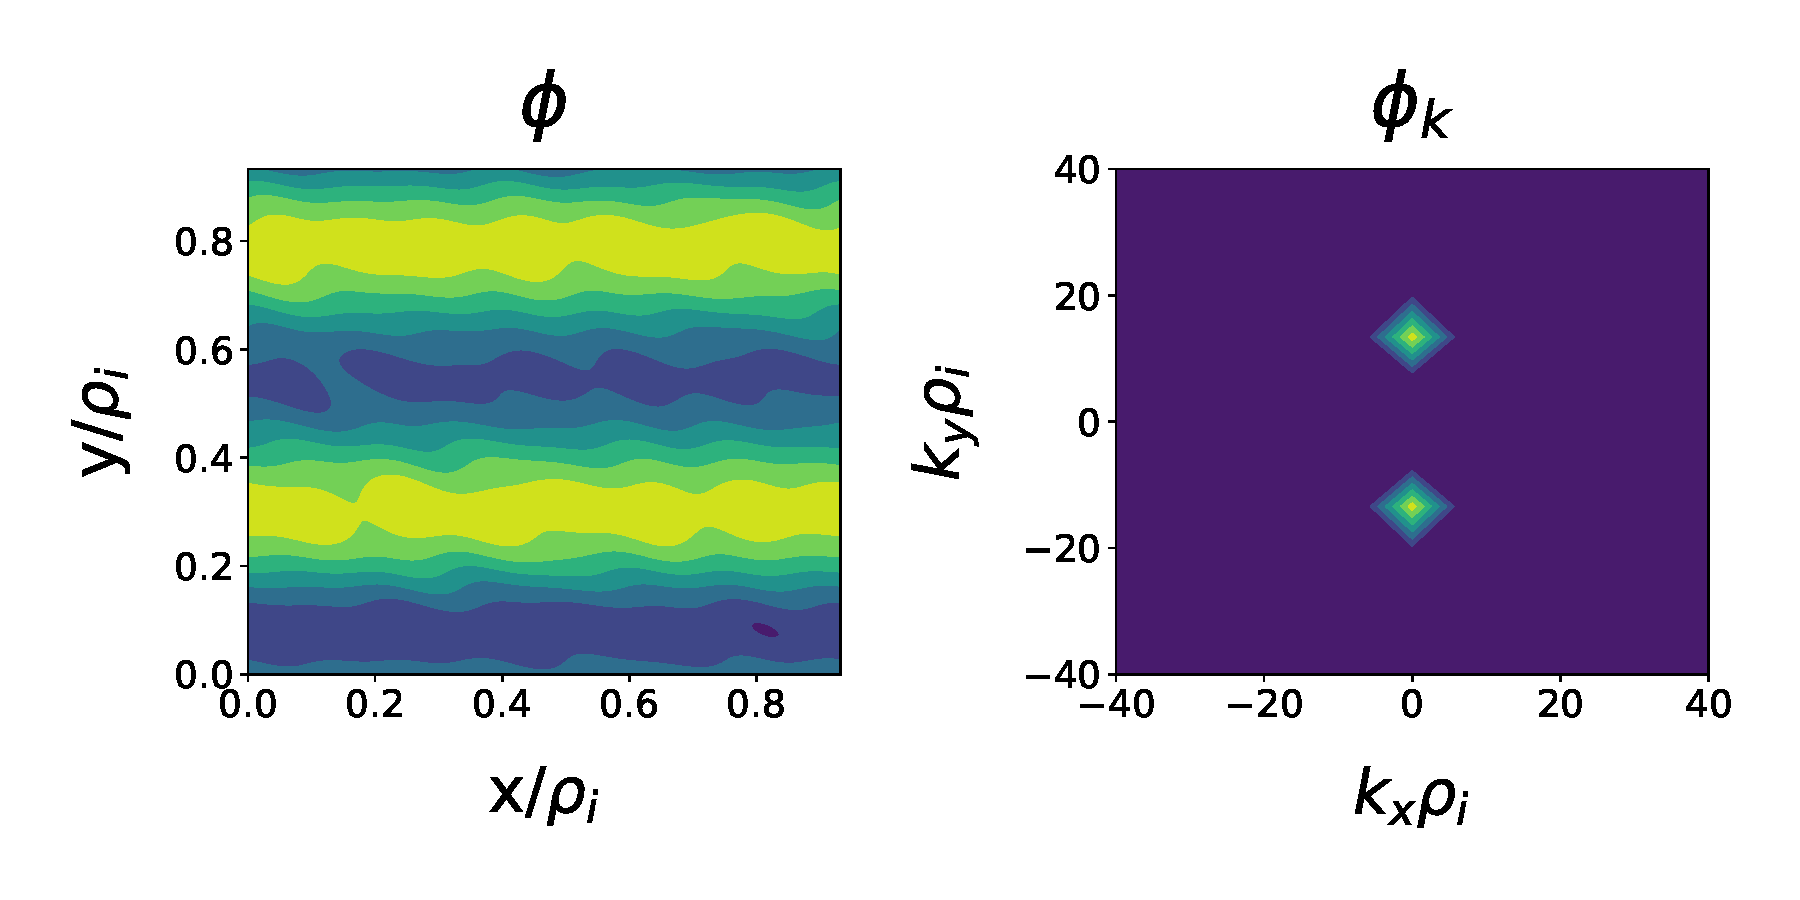
\includegraphics[height=.43\textheight, width=\textwidth]{Images/hmPhiETG_init.pdf}
               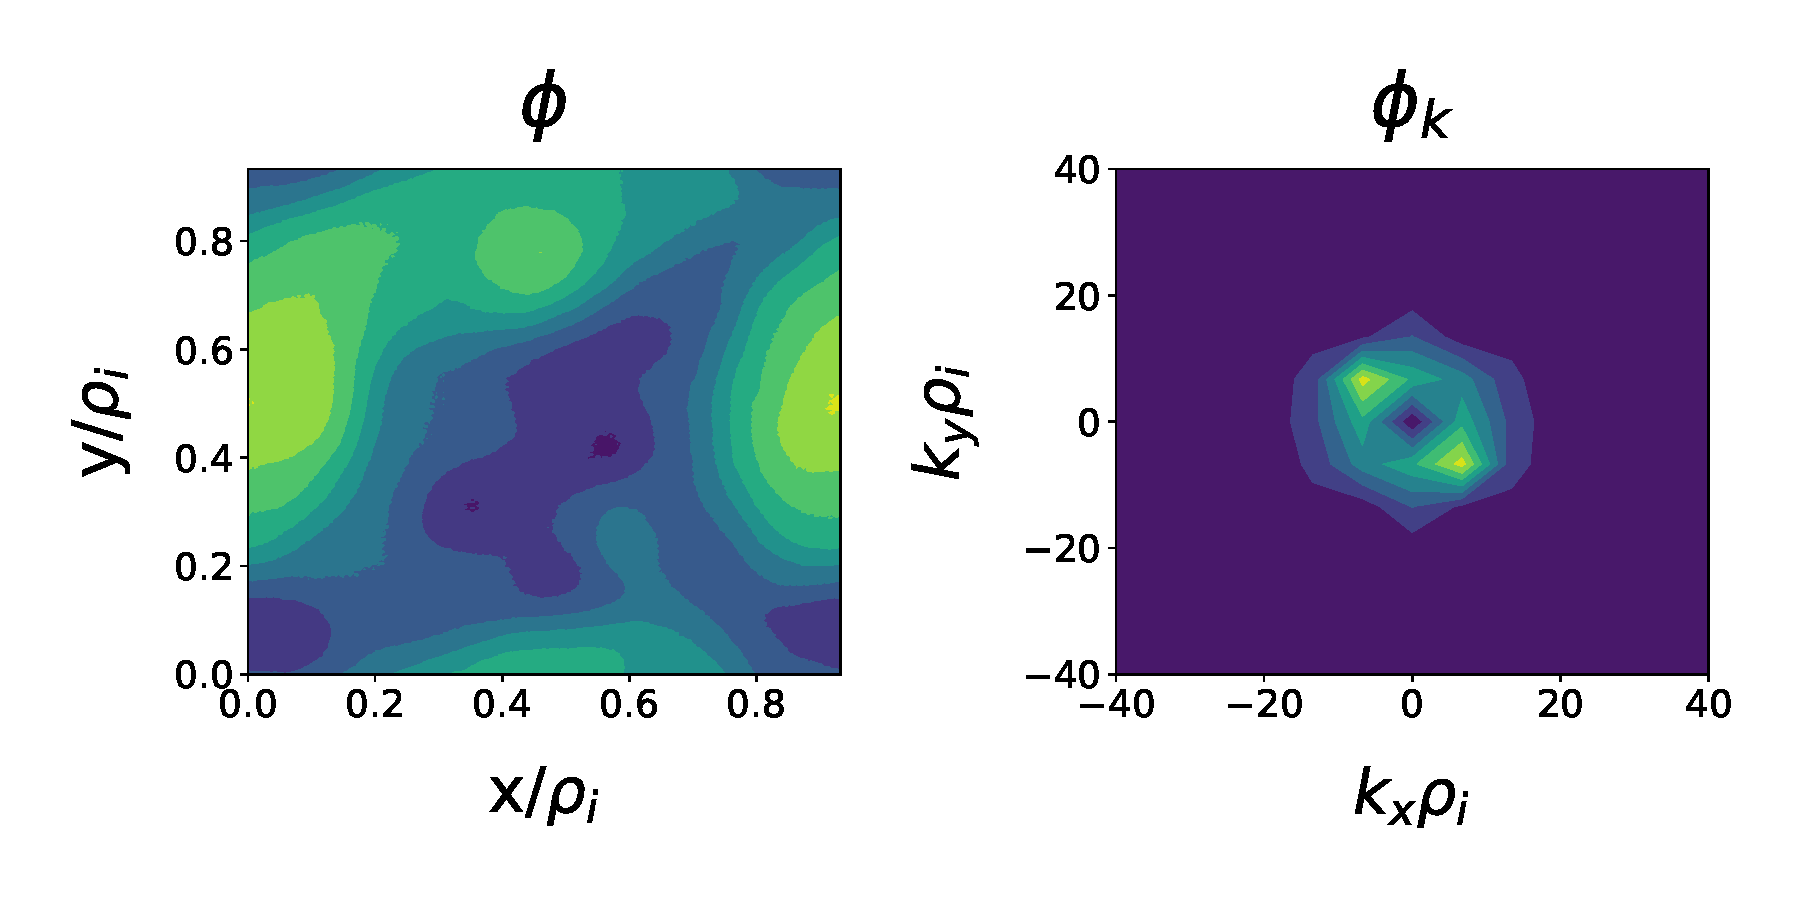
\includegraphics[height=.43\textheight, width=\textwidth]{Images/hmPhiETG_iso.pdf}
            \end{figure}
         \column{0.3\textwidth}
            \begin{itemize}
               \vspace*{-1cm}
               \item Results of H-M code. Initial condition (above) isotropizes at later time (below).
               \item Add parameters?
            \end{itemize}
      \end{columns}
   \end{frame}

   \begin{frame}{GENE ETG Streamer Test}
      \begin{columns}
         \column{0.7\textwidth}
            \begin{figure}
               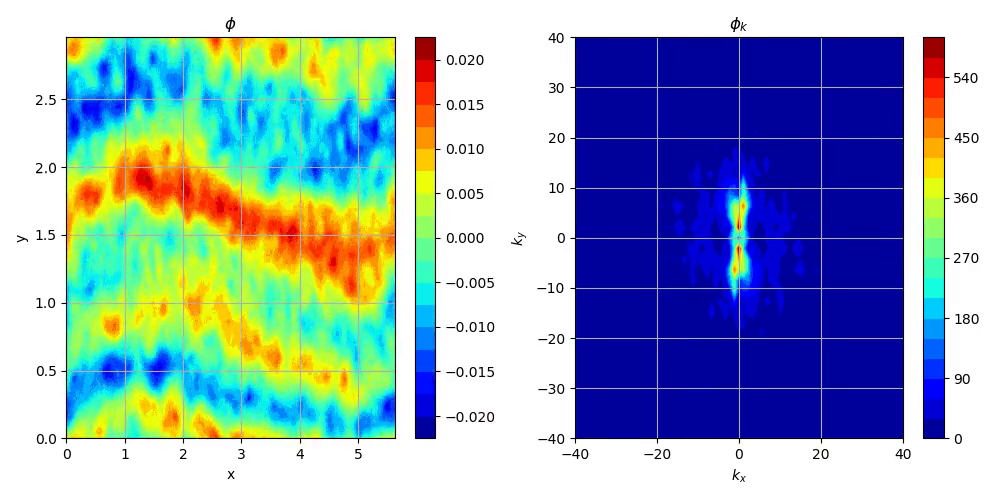
\includegraphics[height=.4\textheight,width=\textwidth]{Images/hmETG_geneInit.png}
               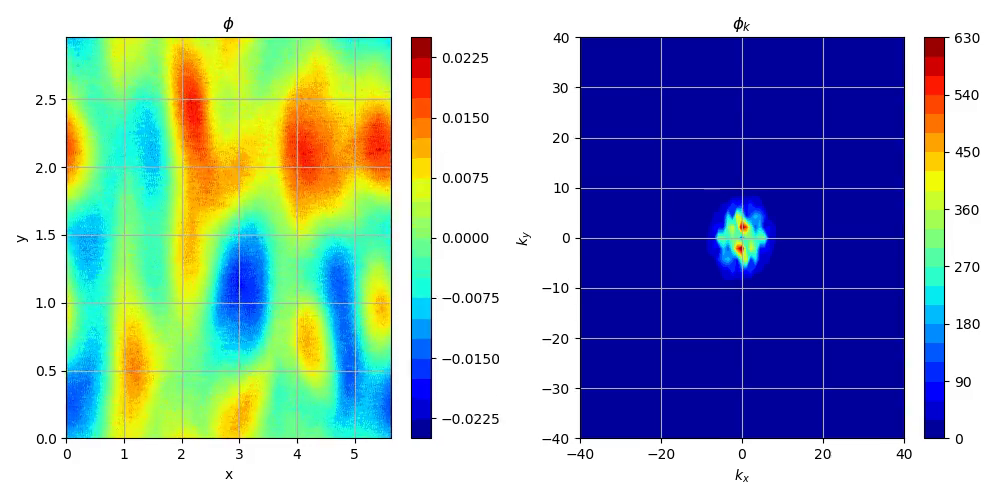
\includegraphics[height=.4\textheight,width=\textwidth]{Images/hmETG_geneIso.png}
            \end{figure}
         \column{0.3\textwidth}
            \begin{itemize}
               \item Test of GENE saturated ETG results into H-M code. Initial conditions (above) isotropize at later times (below).
               \item Inverse energy cascade observed.
            \end{itemize}
      \end{columns}
   \end{frame}

   \section{Zonal Flow Excitation}

   \begin{frame}{Zonal Flow Excitation}
      \begin{columns}
         \column{0.6\textwidth}
            \begin{figure}
               \vspace*{-.6cm}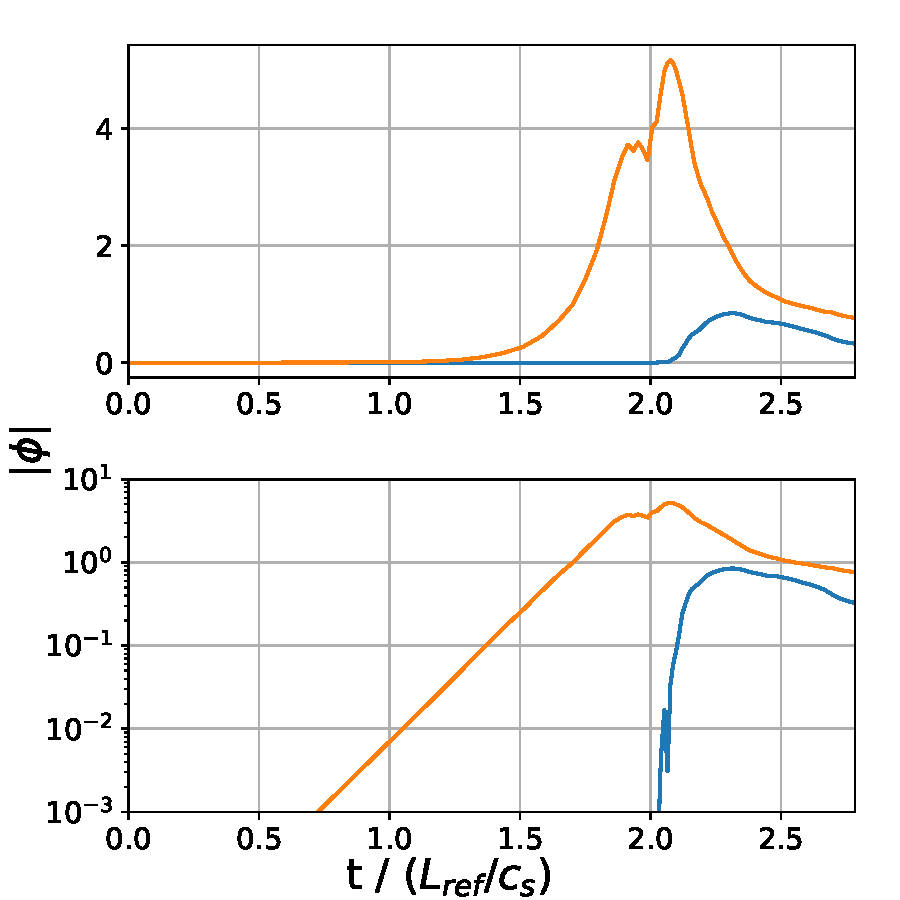
\includegraphics[scale=.35]{Images/zonalFlow.pdf}
               \caption{A non-linear GENE sim initialized with two modes - a default ZF mode ($k_y=0$) and
                        the orange ETG ($k_y\rho_i=6.36$) mode. This excites the blue ZF mode ($k_y=0,k_x\rho_i=4.955$).}
            \end{figure}
         \column{0.4\textwidth}
            \vspace*{-.5cm}
            \begin{itemize}
               \item Zonal flow can be spontaneously excited by intermediate-scale ETG turbulence in tokamak geometries - 
               $k_{\perp}\rho_e \ll 1 \ll k_{\perp}\rho_i$.
               \item Plan to carry out large-scale ETG simulations with GENE to compare to theory of zonal flow excitation by ETG modes.
            \end{itemize}
      \end{columns}
   \end{frame}
   
   \section*{References}
      %\nocite{Djairo} \nocite{PhilPanof} \nocite{Fleming} \nocite{Shankar}
      \begin{frame}{References}
          %\printbibliography
      \end{frame}

\end{document}